\documentclass[11pt,a4paper]{report}

\usepackage[utf8]{inputenc}
\usepackage[T1]{fontenc}
\usepackage{lmodern}
\usepackage[margin=2.5cm]{geometry}
\usepackage{graphicx}
\usepackage{booktabs}
\usepackage{tabularx}
\usepackage{xcolor}
\usepackage{listings}
\usepackage{tikz}
\usetikzlibrary{positioning,arrows.meta,shapes.geometric,fit,backgrounds}
\usepackage{pgfplots}
\pgfplotsset{compat=1.18}
\usepackage{hyperref}
\usepackage{enumitem}
\usepackage{caption}
\usepackage{fancyhdr}

\hypersetup{colorlinks=true, linkcolor=blue!50!black, urlcolor=blue!50!black, citecolor=blue!50!black}

\definecolor{codebg}{HTML}{F4F6FA}
\definecolor{kw}{HTML}{1F4E9A}
\definecolor{str}{HTML}{8A3B12}
\definecolor{cmt}{HTML}{5B6B7F}
\lstset{
  basicstyle=\ttfamily\footnotesize, backgroundcolor=\color{codebg}, frame=single, rulecolor=\color{black!15},
  keywordstyle=\color{kw}\bfseries, stringstyle=\color{str}, commentstyle=\color{cmt}\itshape,
  breaklines=true, columns=fullflexible, showstringspaces=false, xleftmargin=4pt, xrightmargin=4pt,
}
\lstdefinelanguage{Cypher}{
  morekeywords={MATCH,WHERE,RETURN,DISTINCT,WITH,UNWIND,MERGE,SET,CALL,YIELD,ORDER,BY,LIMIT,CONTAINS,AND,OR,AS,count,collect,DETACH,DELETE,OPTIONAL},
  sensitive=true, morestring=[b]', morestring=[b]"
}

\pagestyle{fancy}
\fancyhf{}
\fancyhead[L]{\small AI-powered knowledge graph analytics platform}
\fancyhead[R]{\small INPT -- Innovation \& AMOA}
\fancyfoot[C]{\thepage}

\newcommand{\RQ}[1]{\textbf{RQ#1}}

\begin{document}

% ---------------------------------------------------------------- title page
\begin{titlepage}
  \centering
  {\large\scshape Institut National des Postes et T\'el\'ecommunications (INPT)\par}
  \vspace{0.3cm}
  {\scshape 3\textsuperscript{rd} year -- Innovation \& AMOA\par}
  \vspace{3cm}
  \rule{\linewidth}{0.6pt}\par\vspace{0.4cm}
  {\Huge\bfseries AI-powered Knowledge Graph\\[0.2cm] Analytics Platform\par}
  \vspace{0.4cm}
  {\Large Big Data, LLM extraction, Neo4j and GraphRAG:\\ a comparative evaluation\par}
  \vspace{0.3cm}
  \rule{\linewidth}{0.6pt}\par
  \vspace{2.5cm}
  {\large Project report -- Big Data Analytics\par}
  \vspace{2cm}
  {\large\textbf{Authors}\par}
  \vspace{0.3cm}
  {\Large Azzeddine Abouaam\par}
  \vspace{0.15cm}
  {\Large Zakaria Ezzaami\par}
  \vfill
  {\large Academic year 2026--2027\par}
\end{titlepage}

% ---------------------------------------------------------------- abstract
\begin{abstract}
This report presents the design, implementation and evaluation of an AI-powered knowledge graph analytics
platform. Information is collected from heterogeneous sources (websites, a REST API, PDF and Word
documents, e-mails, plain-text files and a relational database), stored in HDFS, and converted into entities and
relationships by a large language model (LLM). A rule-based entity-resolution step and a Spark ETL job validate,
deduplicate and load the result into a Neo4j knowledge graph. On top of this single graph we compare two analytical
approaches: \emph{structured graph analytics} (Cypher queries and Neo4j Graph Data Science algorithms) and
\emph{GraphRAG} (graph retrieval combined with LLM generation). The whole system runs as a Docker Compose
proof of concept with a local, CPU-only model (\texttt{qwen2.5:3b}).

On a hand-annotated benchmark of 12 questions, the LLM extracts entities with an F1 of 0.86 and relations with an
F1 of 0.71 after schema validation. Entity resolution removes every duplicate node and doubles Cypher accuracy on
multi-hop questions (0.17 to 0.33). Cypher answers in about 10\,ms with no inference cost and wins on aggregation;
GraphRAG takes about 57\,s and 1\,200 tokens per question but wins on semantic questions and can answer from entity
descriptions when an edge is missing. Every answer is backed by source citations, none of them invalid.
\end{abstract}

\tableofcontents

% ================================================================ 1
\chapter{Introduction}

\section{Context}
Organizations hold knowledge scattered across web pages, reports, e-mails, office documents and databases. The
facts that matter most -- who leads which company, who invested in whom, which supplier serves which customer --
are rarely stored in one place, and answering a question often requires connecting facts found in different
documents (\emph{multi-hop} reasoning). Knowledge graphs model this naturally: entities become nodes and facts
become typed edges. Two recent developments make building and querying such graphs much cheaper:
\begin{itemize}
  \item \textbf{LLM-based information extraction}, which turns unstructured text into entities and relations
        without task-specific training;
  \item \textbf{GraphRAG}, which retrieves a relevant subgraph and lets an LLM answer natural-language questions
        over it, instead of requiring the user to write a query language.
\end{itemize}

\section{Objectives}
The goal of the project is to collect information from heterogeneous sources, extract entities and relationships,
build a knowledge graph, and \textbf{compare traditional graph analytics with LLM-based graph retrieval and
reasoning}. The key design principle is to maintain \emph{one knowledge graph supporting two analytical approaches},
so that the comparison is fair: both approaches use exactly the same underlying data.

\section{Research questions}
\begin{description}[leftmargin=1.4cm,style=nextline]
  \item[\RQ{1}] How accurately can an LLM extract entities and relationships from heterogeneous documents?
  \item[\RQ{2}] How does entity resolution affect the quality of the resulting knowledge graph?
  \item[\RQ{3}] How does GraphRAG perform compared with direct Cypher queries for multi-hop and semantic questions?
  \item[\RQ{4}] What trade-offs exist between answer quality, completeness, latency and inference cost?
  \item[\RQ{5}] How can source provenance improve the reliability and explainability of generated answers?
\end{description}

\section{Report structure}
Chapter~\ref{ch:archi} describes the architecture. Chapter~\ref{ch:impl} details the implementation, phase by
phase. Chapter~\ref{ch:data} presents the dataset and ground truth, Chapter~\ref{ch:eval} the evaluation method and
Chapter~\ref{ch:results} the results. Chapter~\ref{ch:discussion} discusses trade-offs, limitations and responsible
use, and Chapter~\ref{ch:conclusion} concludes.

% ================================================================ 2
\chapter{Architecture}\label{ch:archi}

\section{Overview}
Figure~\ref{fig:archi} shows the data flow. Sources are collected by a crawler and landed in HDFS. An LLM
extracts entities and relations, which are resolved and then validated, deduplicated and transformed by Spark before
being loaded into Neo4j. The graph then feeds two branches -- graph analytics and GraphRAG -- whose outputs are
compared by the evaluation module.

\begin{figure}[ht]
\centering
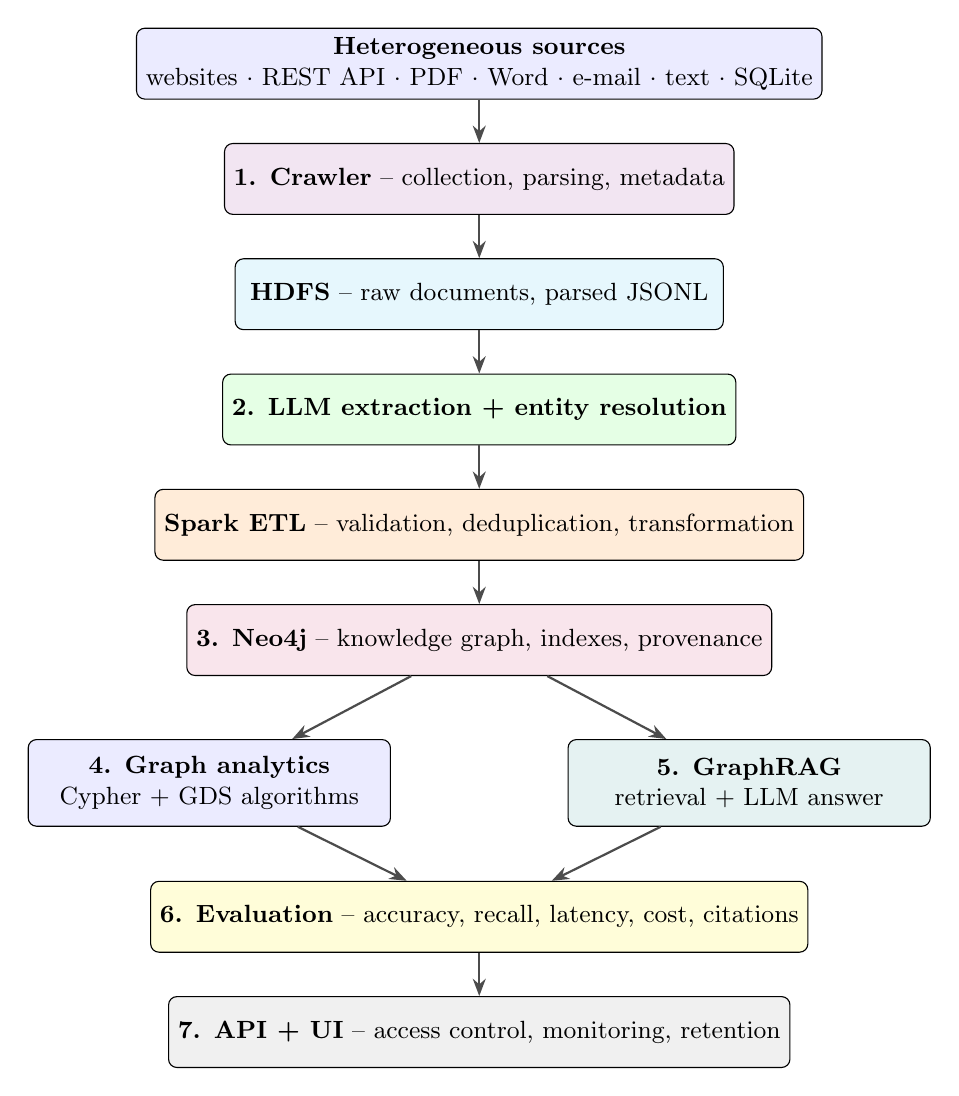
\begin{tikzpicture}[
  node distance=0.55cm and 0.6cm,
  box/.style={draw, rounded corners=3pt, align=center, minimum width=6.2cm, minimum height=0.9cm, font=\small},
  src/.style={box, fill=blue!8},
  ing/.style={box, fill=violet!10},
  store/.style={box, fill=cyan!10},
  llm/.style={box, fill=green!10},
  spark/.style={box, fill=orange!15},
  graph/.style={box, fill=purple!10},
  half/.style={draw, rounded corners=3pt, align=center, minimum width=4.6cm, minimum height=1.1cm, font=\small},
  arr/.style={-{Stealth[length=2.2mm]}, thick, black!70}
]
\node[src] (s) {\textbf{Heterogeneous sources}\\ websites $\cdot$ REST API $\cdot$ PDF $\cdot$ Word $\cdot$ e-mail $\cdot$ text $\cdot$ SQLite};
\node[ing, below=of s] (c) {\textbf{1. Crawler} -- collection, parsing, metadata};
\node[store, below=of c] (h) {\textbf{HDFS} -- raw documents, parsed JSONL};
\node[llm, below=of h] (l) {\textbf{2. LLM extraction + entity resolution}};
\node[spark, below=of l] (sp) {\textbf{Spark ETL} -- validation, deduplication, transformation};
\node[graph, below=of sp] (n) {\textbf{3. Neo4j} -- knowledge graph, indexes, provenance};
\node[half, fill=blue!8, below left=0.8cm and -2.6cm of n] (ga) {\textbf{4. Graph analytics}\\ Cypher + GDS algorithms};
\node[half, fill=teal!10, below right=0.8cm and -2.6cm of n] (gr) {\textbf{5. GraphRAG}\\ retrieval + LLM answer};
\node[box, fill=yellow!15, below=2.6cm of n] (e) {\textbf{6. Evaluation} -- accuracy, recall, latency, cost, citations};
\node[box, fill=gray!12, below=of e] (api) {\textbf{7. API + UI} -- access control, monitoring, retention};
\draw[arr] (s) -- (c); \draw[arr] (c) -- (h); \draw[arr] (h) -- (l); \draw[arr] (l) -- (sp); \draw[arr] (sp) -- (n);
\draw[arr] (n) -- (ga); \draw[arr] (n) -- (gr); \draw[arr] (ga) -- (e); \draw[arr] (gr) -- (e); \draw[arr] (e) -- (api);
\end{tikzpicture}
\caption{Platform architecture: one knowledge graph, two analytical approaches.}
\label{fig:archi}
\end{figure}

\section{Technology stack and deployment}
The proof of concept is a single Docker Compose project. Table~\ref{tab:services} lists the services.

\begin{table}[ht]
\centering
\small
\begin{tabularx}{\linewidth}{lllX}
\toprule
\textbf{Service} & \textbf{Image} & \textbf{Port} & \textbf{Role} \\
\midrule
\texttt{namenode} & \texttt{apache/hadoop:3.4.1} & 9870 & HDFS NameNode (WebHDFS API, web UI) \\
\texttt{datanode} & \texttt{apache/hadoop:3.4.1} & -- & HDFS DataNode (replication 1) \\
\texttt{neo4j} & \texttt{neo4j:5-community} & 7474, 7687 & Graph database + Graph Data Science plugin \\
\texttt{ollama} & \texttt{ollama/ollama} & -- & Local LLM server, OpenAI-compatible API \\
\texttt{website} & \texttt{python:3.12-slim} & -- & Demo website and JSON API crawled by the platform \\
\texttt{app} & custom (Python 3.12, Java 21) & 8080 & Crawler, extraction, Spark ETL, analytics, GraphRAG, evaluation, API/UI \\
\bottomrule
\end{tabularx}
\caption{Docker Compose services.}
\label{tab:services}
\end{table}

The application image bundles PySpark~4.0 with a Java~21 runtime so that the Spark job runs next to the
Python services. The LLM is accessed through an OpenAI-compatible endpoint: by default a local Ollama server running
\texttt{qwen2.5:3b}, but any compatible provider can be used by setting \texttt{LLM\_BASE\_URL} and
\texttt{LLM\_MODEL}.

\section{Graph schema}
A shared, explicit schema constrains both the LLM and the validation step (Table~\ref{tab:schema}). Every entity
carries the label \texttt{Entity} plus its type label, a \texttt{description} and the list of source documents.
Every relation carries \texttt{sources}, \texttt{evidence} (quotes from the text), \texttt{confidence} and
\texttt{mentions}. Documents are nodes too, linked by \texttt{MENTIONED\_IN}.

\begin{table}[ht]
\centering
\small
\begin{tabular}{lll}
\toprule
\textbf{Relation} & \textbf{Source type} & \textbf{Target type} \\
\midrule
\texttt{FOUNDED}, \texttt{LEADS}, \texttt{WORKS\_FOR}, \texttt{BOARD\_MEMBER\_OF} & Person & Organization \\
\texttt{INVESTED\_IN}, \texttt{ACQUIRED}, \texttt{SUPPLIES} & Organization & Organization \\
\texttt{PARTNERS\_WITH} (symmetric) & Organization & Organization \\
\texttt{DEVELOPS} & Organization & Product \\
\texttt{LOCATED\_IN} & Organization & Location \\
\bottomrule
\end{tabular}
\caption{Relation types and their type signatures (entity types: Person, Organization, Product, Location).}
\label{tab:schema}
\end{table}

% ================================================================ 3
\chapter{Implementation}\label{ch:impl}
The implementation follows the seven phases of the project roadmap (Table~\ref{tab:phases}).

\begin{table}[ht]
\centering
\small
\begin{tabularx}{\linewidth}{clXl}
\toprule
\textbf{Phase} & \textbf{Scope} & \textbf{Deliverable} & \textbf{Module} \\
\midrule
1 & Sample documents, crawler, HDFS & Working ingestion pipeline & \texttt{crawler.py} \\
2 & LLM extraction, entity resolution & Structured entities and relationships & \texttt{extract.py}, \texttt{resolve.py} \\
3 & Spark transformations, Neo4j ingestion & Populated knowledge graph & \texttt{spark\_etl.py} \\
4 & Cypher queries, graph algorithms & Graph analytics module & \texttt{analytics.py} \\
5 & GraphRAG retrieval and generation & Natural-language graph assistant & \texttt{graphrag.py} \\
6 & Ground truth, comparative tests & Benchmark report & \texttt{evaluate.py} \\
7 & API, interface, monitoring, access control & Integrated application & \texttt{api.py} \\
\bottomrule
\end{tabularx}
\caption{Roadmap phases and corresponding modules.}
\label{tab:phases}
\end{table}

\section{Phase 1 -- Collection and HDFS storage}
The crawler handles every source family of the architecture:
\begin{itemize}
  \item \textbf{Websites}: breadth-first crawl from seed URLs, restricted to the seeds' hosts, using the standard
        library HTML parser to extract the title, visible text and links;
  \item \textbf{APIs}: each item of a JSON array becomes one document;
  \item \textbf{Files}: PDF (\texttt{pypdf}), Word (\texttt{python-docx}), e-mail (\texttt{email} standard library,
        headers kept as metadata) and plain text;
  \item \textbf{Databases}: each row of each SQLite table becomes a \emph{column: value} document.
\end{itemize}
Each document receives a stable identifier (e.g.\ \texttt{pdf:northwind\_report.pdf}), a SHA-256 hash used for
deduplication, and a collection timestamp. Original bytes are written to \texttt{/raw/<kind>/} and parsed documents to
\texttt{/parsed/docs.jsonl} through the WebHDFS REST API. The run collected 12 documents from 7 source kinds.

\section{Phase 2 -- LLM extraction and entity resolution}
\paragraph{Extraction.} One LLM call per document, at temperature 0 and in JSON mode. The prompt lists the
allowed entity and relation types with their direction, requires an \emph{evidence} quote and a \emph{confidence}
for every relation, and gives one worked example. A first version of the prompt without the example produced many
reversed relations (``Helios Robotics FOUNDED Amara Okafor'') and no locations; adding the one-shot example fixed
most of them.

\paragraph{Entity resolution.} Surface forms are clustered with a union-find structure over cleaned names
(honorifics such as \emph{Dr.} and legal suffixes such as \emph{SA}, \emph{LLP} or \emph{S.p.A.} removed). Two names
are merged when:
\begin{enumerate}
  \item their normalized keys are identical (\emph{Helios Robotics SA} = \emph{Helios Robotics});
  \item one name's tokens are contained in exactly one other name (\emph{Helios} $\to$ \emph{Helios Robotics});
        ambiguous containment is not merged;
  \item they match by initials (\emph{A. Okafor} $\to$ \emph{Amara Okafor});
  \item their spelling is nearly identical (\texttt{difflib} ratio $\geq 0.92$).
\end{enumerate}
The canonical name is the most frequent cleaned form. On the corpus, 28 surface names were reduced to 20 entities.
Both a resolved and an unresolved version are written to HDFS so that the effect of resolution can be measured.

\section{Phase 3 -- Spark ETL and Neo4j ingestion}
The Spark job reads the extracted JSONL from HDFS and performs three steps:
\begin{itemize}
  \item \textbf{Validation}: relation types are normalized (\emph{CEO} $\to$ \texttt{LEADS}); relations that violate
        the type signature are \emph{repaired} by swapping source and target when the reversed direction fits,
        and dropped otherwise; self-loops are removed;
  \item \textbf{Deduplication}: one node per name (majority type vote), one edge per (source, type, target), with the
        union of source documents, all evidence quotes, the maximum confidence and the mention count;
  \item \textbf{Transformation and loading}: the curated layer is written as Parquet to HDFS, then loaded into Neo4j
        with batched \texttt{UNWIND ... MERGE} statements executed in parallel from Spark partitions.
\end{itemize}

\begin{lstlisting}[language=Python, caption={Schema validation with direction repair (shared by Spark and the evaluator).}]
want_s, want_t = SIGNATURES[t]
def fits(a, b):  # unknown endpoint types (None) are accepted
    return a in (None, want_s) and b in (None, want_t)
if not fits(st, dt):
    if not fits(dt, st):
        return None            # cannot fit the schema: drop
    src, dst = dst, src        # reversed by the LLM: repair
\end{lstlisting}

Neo4j constraints guarantee unique entity names and document ids, and a full-text index covers entity names and
descriptions for retrieval. The run produced 20 entity nodes and 24 deduplicated edges from 29 extracted relations.

\section{Phase 4 -- Graph analytics}
The analytics module exposes direct Cypher queries and Graph Data Science algorithms on an in-memory projection of
the entity graph:
\begin{itemize}
  \item \textbf{Overview} and \textbf{degree centrality};
  \item \textbf{PageRank} -- most influential entities (Helios Robotics, Verdant Grid, Northwind Capital);
  \item \textbf{Betweenness} -- brokers connecting otherwise distant parts of the graph (Northwind Capital, the
        investor, ranks first);
  \item \textbf{Louvain communities} -- three clusters were found: the Verdant Grid / Corvid Analytics ecosystem, the
        Helios Robotics / Northwind cluster, and the Lumen Batteries / Quanta Bio cluster;
  \item \textbf{Shortest paths} with provenance, e.g.\ Mei Tanaka $\to$ Corvid Analytics $\to$ Verdant Grid
        $\leftarrow$ Northwind Capital, each hop listing its source documents.
\end{itemize}

\section{Phase 5 -- GraphRAG}
GraphRAG answers a natural-language question in three steps:
\begin{enumerate}
  \item \textbf{Seed retrieval}: content words of the question (stop words removed, fuzzy matching for longer words)
        query the full-text index; seeds scoring below half of the best score are discarded, because a small model
        loses track of the question when the context covers the whole graph;
  \item \textbf{Subgraph expansion}: all relations within two hops of the seeds, one-hop facts first, with their
        sources, evidence and confidence, plus the descriptions of the entities involved;
  \item \textbf{Generation}: the LLM answers using only these facts, cites source ids in brackets after each claim,
        and presents facts as claims from sources rather than verified truth. Cited ids are checked against the
        retrieved context.
\end{enumerate}

\section{Phase 6 -- Evaluation module}
\texttt{evaluate.py} computes extraction metrics against the gold annotations, measures the resolution ablation,
then loads the unresolved and the resolved graph in turn and runs every benchmark question through both approaches.
Results are written to \texttt{reports/benchmark.json} and \texttt{reports/benchmark.md}.

\section{Phase 7 -- Integrated application}
A FastAPI service exposes the platform through a REST API and a minimal web interface:
\begin{itemize}
  \item \texttt{POST /ask} (GraphRAG), \texttt{GET /analytics/\{name\}}, \texttt{GET /path}, \texttt{GET /entity};
  \item \textbf{access control}: API keys mapped to \emph{reader} and \emph{admin} roles (401 without a key, 403 for an
        insufficient role), every request audit-logged, question length validated;
  \item \textbf{monitoring}: \texttt{/health} probes Neo4j and HDFS; \texttt{/metrics} exposes request counts,
        latencies and LLM token usage in Prometheus format;
  \item \textbf{data retention}: \texttt{POST /admin/retention} deletes documents older than a configurable number of
        days, then every fact and entity no longer backed by any source.
\end{itemize}

% ================================================================ 4
\chapter{Dataset and ground truth}\label{ch:data}

\section{Corpus}
To evaluate the platform without processing data about real people, we built an \textbf{entirely fictional} corpus
describing a small European technology ecosystem (Table~\ref{tab:corpus}). It was designed to stress the two
difficult points of the pipeline:
\begin{itemize}
  \item \textbf{facts spread across sources}: answering most multi-hop questions requires combining at least two
        documents of different formats;
  \item \textbf{inconsistent naming}: the same entity appears as \emph{Dr.\ Amara Okafor}, \emph{Okafor} or
        \emph{A.\ Okafor}, and \emph{Northwind Capital Partners LLP}, \emph{Northwind Capital} or \emph{Northwind}.
\end{itemize}

\begin{table}[ht]
\centering
\small
\begin{tabularx}{\linewidth}{llX}
\toprule
\textbf{Source type} & \textbf{Document(s)} & \textbf{Content} \\
\midrule
Website (crawled) & \texttt{index.html}, \texttt{helios.html}, \texttt{verdant.html} & Company profiles linked from an index page \\
REST API & \texttt{news.json} (3 items) & Investment and partnership news \\
PDF & \texttt{northwind\_report.pdf} & Investor annual portfolio report \\
Word & \texttt{lumen\_brief.docx} & Battery manufacturer company brief \\
E-mail & \texttt{corvid\_partnership.eml} & Partnership announcement from a founder \\
Text file & \texttt{basel\_notes.txt} & Field notes \\
Database & \texttt{registry.sqlite} (2 rows) & Company registry table \\
\bottomrule
\end{tabularx}
\caption{Fictional sample corpus: 12 documents from 7 source types.}
\label{tab:corpus}
\end{table}

\section{Ground truth}
The gold file contains 24 entities with their aliases, 28 relations and 12 questions. Each question has its type,
gold answer (with accepted variants), supporting source documents, a reference Cypher query (the \emph{graph
analytics} approach) and, for multi-hop questions, the gold path. Table~\ref{tab:questions} lists the questions.

\begin{table}[ht]
\centering
\small
\begin{tabularx}{\linewidth}{llXl}
\toprule
\textbf{Id} & \textbf{Type} & \textbf{Question} & \textbf{Answer} \\
\midrule
Q1 & single-hop & Who founded Helios Robotics? & Amara Okafor \\
Q2 & single-hop & In which city is Verdant Grid headquartered? & Oslo \\
Q3 & single-hop & Which companies has Northwind Capital invested in? & Helios, Verdant, Lumen \\
Q4 & aggregation & How many companies has Northwind Capital invested in? & 3 \\
Q5 & multi-hop & In which city is the battery supplier of Helios Robotics located? & Turin \\
Q6 & multi-hop & Who leads the company that partners with Corvid Analytics? & Lars Henriksen \\
Q7 & multi-hop & Which board member of Helios Robotics works for one of its investors? & Daniel Weiss \\
Q8 & multi-hop & Who founded the company that partners with the developer of GridMind? & Mei Tanaka \\
Q9 & multi-hop & Which company did the developer of GridMind acquire, and where is it based? & Kestrel, Bergen \\
Q10 & multi-hop & Which company supplies two different companies Northwind invested in? & Lumen Batteries \\
Q11 & semantic & Which company works on energy storage technology? & Lumen Batteries \\
Q12 & semantic & Which organization automates biotech laboratories with robots? & Quanta Bio \\
\bottomrule
\end{tabularx}
\caption{Benchmark questions.}
\label{tab:questions}
\end{table}

\begin{lstlisting}[language=Cypher, caption={Reference Cypher query for the multi-hop question Q7.}]
MATCH (p:Person)-[:BOARD_MEMBER_OF]->(h:Entity),
      (p)-[:WORKS_FOR]->(i:Entity)-[:INVESTED_IN]->(h)
WHERE toLower(h.name) CONTAINS 'helios'
RETURN DISTINCT p.name
\end{lstlisting}

% ================================================================ 5
\chapter{Evaluation methodology}\label{ch:eval}

\begin{itemize}
  \item \textbf{Extraction (\RQ{1})}: precision, recall and F1 of entities and relations against the gold
        annotations. Extracted names are mapped to gold entities through the alias table (lenient matching), so that
        this metric isolates the LLM's extraction quality from naming. Relations are measured twice: as returned by
        the LLM and after Spark schema validation.
  \item \textbf{Entity resolution (\RQ{2})}: on the unresolved and resolved graphs, number of nodes, duplicate nodes
        (several nodes for one gold entity), fragmentation (nodes per gold entity) and \emph{walkable multi-hop
        paths}: a gold path counts only if its hops are connected through \emph{identical} nodes, i.e.\ if a graph
        traversal could actually follow it. QA accuracy is also measured on both graphs.
  \item \textbf{Question answering (\RQ{3})}: for each question, a gold item is found if one of its accepted forms
        appears (whole word, case-insensitive) in the answer. \emph{Recall} is the share of gold items found;
        a question is \emph{correct} when recall is 1. Cypher results and GraphRAG answers are scored the same way.
  \item \textbf{Cost (\RQ{4})}: end-to-end latency per question and LLM tokens, at extraction and query time.
  \item \textbf{Provenance (\RQ{5})}: share of answers with citations, invalid citations (ids not present in the
        retrieved context) and citation precision (share of cited documents that are gold supporting documents).
\end{itemize}
All experiments ran on a laptop CPU (8 cores, no GPU) with \texttt{qwen2.5:3b} at temperature 0.

% ================================================================ 6
\chapter{Results}\label{ch:results}

\section{\RQ{1} -- Extraction accuracy}
\begin{table}[ht]
\centering
\begin{tabular}{lcccccc}
\toprule
\textbf{Level} & \textbf{Precision} & \textbf{Recall} & \textbf{F1} & \textbf{TP} & \textbf{Predicted} & \textbf{Gold} \\
\midrule
Entities & 1.000 & 0.750 & 0.857 & 18 & 18 & 24 \\
Relations (LLM output) & 0.692 & 0.643 & 0.667 & 18 & 26 & 28 \\
Relations (after validation) & 0.783 & 0.643 & 0.706 & 18 & 23 & 28 \\
\bottomrule
\end{tabular}
\caption{Extraction quality of \texttt{qwen2.5:3b}.}
\label{tab:rq1}
\end{table}

Entity extraction is precise (no false entity) but misses a quarter of the gold entities, mostly cities mentioned
indirectly (``an Oslo-based company'') and secondary mentions. Relation extraction is the weaker step: the model
confuses relation types (Daniel Weiss \texttt{LEADS} instead of \texttt{WORKS\_FOR} Northwind) and sometimes reverses
directions. Spark validation drops or repairs schema-violating relations, raising relation precision from 0.69 to
0.78 at no cost in recall.

\section{\RQ{2} -- Effect of entity resolution}
\begin{table}[ht]
\centering
\small
\begin{tabular}{lcccccc}
\toprule
\textbf{Graph} & \textbf{Nodes} & \textbf{Gold-matched} & \textbf{Gold found} & \textbf{Duplicates} & \textbf{Fragm.} & \textbf{Walkable} \\
\midrule
Unresolved & 28 & 26 & 20 & 6 & 1.30 & 1/6 \\
Resolved & 20 & 20 & 20 & 0 & 1.00 & 2/6 \\
\bottomrule
\end{tabular}
\caption{Graph quality with and without entity resolution.}
\label{tab:rq2}
\end{table}

Resolution removes all six duplicate nodes without merging distinct entities, and doubles the number of gold
multi-hop paths that a traversal can follow. Downstream, Cypher accuracy on multi-hop questions doubles from 0.17
to 0.33 (Table~\ref{tab:rq3}): Q8, for instance, fails on the unresolved graph because \emph{Corvid Analytics} and
\emph{Corvid Analytics Inc.} are two different nodes. The remaining unwalkable paths are caused by relations that
were never extracted, which resolution cannot fix.

\section{\RQ{3} -- Cypher versus GraphRAG}
\begin{table}[ht]
\centering
\small
\begin{tabular}{llccccc}
\toprule
\textbf{Graph} & \textbf{Question type} & \textbf{n} & \multicolumn{2}{c}{\textbf{Cypher}} & \multicolumn{2}{c}{\textbf{GraphRAG}} \\
\cmidrule(lr){4-5}\cmidrule(lr){6-7}
 & & & accuracy & recall & accuracy & recall \\
\midrule
Unresolved & single-hop & 3 & 0.67 & 0.67 & 1.00 & 1.00 \\
 & aggregation & 1 & 1.00 & 1.00 & 0.00 & 0.00 \\
 & multi-hop & 6 & 0.17 & 0.25 & 0.50 & 0.58 \\
 & semantic & 2 & 1.00 & 1.00 & 0.50 & 0.50 \\
 & \textbf{all} & 12 & \textbf{0.50} & 0.54 & \textbf{0.58} & 0.63 \\
\midrule
Resolved & single-hop & 3 & 0.67 & 0.67 & 0.67 & 0.67 \\
 & aggregation & 1 & 1.00 & 1.00 & 0.00 & 0.00 \\
 & multi-hop & 6 & 0.33 & 0.42 & 0.50 & 0.58 \\
 & semantic & 2 & 0.50 & 0.50 & 1.00 & 1.00 \\
 & \textbf{all} & 12 & \textbf{0.50} & 0.54 & \textbf{0.58} & 0.63 \\
\bottomrule
\end{tabular}
\caption{Question-answering accuracy and recall by question type.}
\label{tab:rq3}
\end{table}

\begin{figure}[ht]
\centering
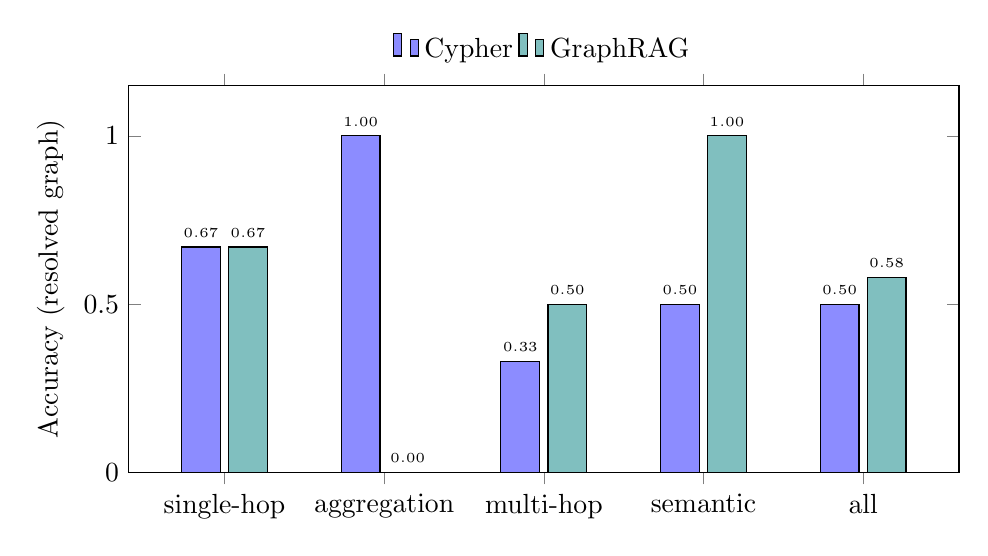
\begin{tikzpicture}
\begin{axis}[
  ybar=3pt, bar width=14pt, width=\linewidth, height=6.5cm,
  ymin=0, ymax=1.15, ylabel={Accuracy (resolved graph)},
  symbolic x coords={single-hop,aggregation,multi-hop,semantic,all}, xtick=data,
  nodes near coords, nodes near coords style={font=\tiny, /pgf/number format/.cd, fixed, fixed zerofill, precision=2},
  legend style={at={(0.5,1.03)}, anchor=south, legend columns=2, draw=none},
  enlarge x limits=0.15,
]
\addplot[fill=blue!45] coordinates {(single-hop,0.67) (aggregation,1.00) (multi-hop,0.33) (semantic,0.50) (all,0.50)};
\addplot[fill=teal!50] coordinates {(single-hop,0.67) (aggregation,0.00) (multi-hop,0.50) (semantic,1.00) (all,0.58)};
\legend{Cypher, GraphRAG}
\end{axis}
\end{tikzpicture}
\caption{Accuracy of both approaches per question type on the resolved graph (automatic, lenient scoring).}
\label{fig:rq3}
\end{figure}

Each approach has clear strengths (Figure~\ref{fig:rq3}):
\begin{itemize}
  \item \textbf{Cypher is exact when the graph is right.} It answers the aggregation question perfectly, while
        GraphRAG over-counts (it listed four investments instead of three). But it is brittle: a single missing or
        mistyped edge on the path returns nothing (Q5, Q6, Q7).
  \item \textbf{GraphRAG is more robust to graph gaps.} Because its context includes entity descriptions, it can
        answer from text even when an edge is missing: Q5 succeeds although the needed edge path is incomplete, and
        both semantic questions are answered, whereas keyword filters in Cypher depend on the exact wording of the
        descriptions.
  \item \textbf{Small-model reasoning is the main limit of GraphRAG.} On Q6, the retrieved context contained the
        answer (Lars Henriksen is described as CEO of Verdant Grid), yet the 3B model chained the wrong hops.
\end{itemize}

\paragraph{Scoring caveat.} The automatic scoring is mention-based and therefore lenient for free-text answers.
Reading the answers on the resolved graph, GraphRAG's answers to Q10 and Q12 mention the gold entity but designate a
different one as the answer. With strict manual judgment, GraphRAG accuracy on the resolved graph is \textbf{5/12
(0.42)}, below Cypher's 6/12 (0.50). Cypher results are lists of values and are not affected.

\section{\RQ{4} -- Latency and cost}
\begin{table}[ht]
\centering
\begin{tabular}{lcc}
\toprule
& \textbf{Cypher} & \textbf{GraphRAG} \\
\midrule
Mean latency per question & $\approx$ 0.01\,s & 57.2\,s \\
LLM tokens per question & 0 & 1\,178 \\
Query authoring & expert writes Cypher & natural language \\
\midrule
\multicolumn{3}{l}{Shared one-off cost -- extraction: 11\,768 tokens, 517\,s of LLM time (43\,s per document)} \\
\bottomrule
\end{tabular}
\caption{Latency and inference cost (resolved graph, CPU only).}
\label{tab:rq4}
\end{table}

Cypher is about four orders of magnitude faster and free at query time, but requires an expert who knows the
schema. GraphRAG trades latency and tokens for accessibility. Both pay the same up-front extraction cost, which
dominates the total for a small number of questions. On a GPU or a hosted model, GraphRAG latency would drop to a few
seconds, but its per-question token cost remains.

\section{\RQ{5} -- Provenance}
All 24 GraphRAG answers (12 per graph) contained citations, and none cited a document absent from the retrieved
context. Citation precision against gold supporting documents was 0.79 on the unresolved graph and 0.54 on the
resolved graph: once entities are merged, each node gathers sources from many documents and the model tends to cite
all of them rather than only the supporting ones. Provenance makes errors \emph{verifiable}: in the Q9 answer, the
model claims Verdant Grid is based in Basel and cites the registry row about Quanta Bio -- a reader following the
citation immediately sees the mistake. Every edge also keeps its evidence quote, which the web interface displays
next to the answer.

% ================================================================ 7
\chapter{Discussion}\label{ch:discussion}

\section{Trade-offs}
\begin{itemize}
  \item \textbf{Quality of the graph bounds both approaches.} Questions Q2 and Q7 fail for both approaches because
        the needed facts were not extracted. Improving extraction (larger model, chunking, multiple passes) helps
        more than improving either query approach.
  \item \textbf{Cypher for precise, repeated, aggregate questions}; \textbf{GraphRAG for exploratory and semantic
        questions} asked by non-experts. A practical system can combine them: GraphRAG for exploration, with
        Cypher (possibly generated by the LLM and validated) for counts and exact lists.
  \item \textbf{Entity resolution is cheap and high-value.} A few dozen lines of rules removed all duplicates and
        doubled walkable multi-hop paths, without any LLM cost.
  \item \textbf{Schema validation is a cheap safety net} for small models: repairing directions raised relation
        precision by 9 points.
\end{itemize}

\section{Limitations}
\begin{itemize}
  \item The corpus is small (12 documents, 28 relations, 12 questions); results show tendencies, not statistically
        robust differences.
  \item Only one, small model was evaluated, because of hardware limits (CPU, about 2\,GB of free memory).
  \item Answer scoring is automatic and lenient for free text (see the scoring caveat above).
  \item Spark runs in local mode inside the application container, with a single HDFS DataNode; the code is
        written for a cluster (\texttt{SPARK\_MASTER}) but was not benchmarked on one.
  \item GraphRAG seeds rely on a full-text index; vector embeddings would improve fuzzy semantic matching.
\end{itemize}

\section{Responsible use}
When a platform of this kind analyzes networks of identifiable people, inferred associations can harm individuals.
The design therefore includes:
\begin{itemize}
  \item a fictional dataset for development and evaluation;
  \item provenance on every node and edge (source documents, evidence quotes, confidence);
  \item a GraphRAG prompt and a user-interface notice presenting answers as claims from cited sources, not verified
        facts;
  \item role-based API keys and audit logging of every request;
  \item a retention endpoint that removes old documents and every fact that depended only on them.
\end{itemize}
Any deployment on real data must restrict collection to lawful, authorized sources.

% ================================================================ 8
\chapter{Conclusion and future work}\label{ch:conclusion}
We built an end-to-end proof of concept of an AI-powered knowledge graph analytics platform: heterogeneous sources
are crawled into HDFS, turned into a knowledge graph by an LLM, entity resolution and Spark, and analyzed in Neo4j by
two approaches that share the same graph. The evaluation answers the five research questions: a small local LLM
extracts entities reliably but relations only moderately well; entity resolution and schema validation are cheap
steps with a large effect; Cypher is fast, exact and best for aggregation, while GraphRAG is slower and costlier but
handles semantic questions and missing edges better; and source provenance makes every generated answer verifiable.

Future work includes:
\begin{itemize}
  \item evaluating larger models (local 7B--14B or hosted) and measuring the quality/cost curve;
  \item a hybrid assistant that generates and validates Cypher for aggregate questions and uses GraphRAG otherwise;
  \item vector embeddings for retrieval and chunking for long documents;
  \item a larger corpus and an LLM-as-judge or human scoring of free-text answers;
  \item a distributed Spark cluster, incremental graph updates, and production authentication (OIDC).
\end{itemize}

% ================================================================ appendix
\appendix
\chapter{Running the platform}

\begin{lstlisting}[language=bash]
docker compose up -d --build                        # HDFS, Neo4j+GDS, Ollama, website, app
docker compose exec ollama ollama pull qwen2.5:3b   # once (~2 GB)
docker compose exec app python pipeline.py          # crawl, extract, resolve, etl, analytics, evaluate
\end{lstlisting}

\begin{itemize}
  \item Web interface and API: \url{http://localhost:8080} (key \texttt{reader-demo-key})
  \item Neo4j Browser: \url{http://localhost:7474}
  \item HDFS NameNode: \url{http://localhost:9870}
  \item Benchmark report: \texttt{reports/benchmark.md}
\end{itemize}

\begin{lstlisting}[language=bash, caption={API examples.}]
K='X-API-Key: reader-demo-key'
curl -H "$K" -H 'Content-Type: application/json' \
     -d '{"question":"Who founded Helios Robotics?"}' localhost:8080/ask
curl -H "$K" localhost:8080/analytics/pagerank
curl -H "$K" 'localhost:8080/path?a=Mei%20Tanaka&b=Northwind'
\end{lstlisting}

\chapter{Project structure}
\begin{lstlisting}
docker-compose.yml   hadoop.env   README.md
app/  crawler.py  extract.py  resolve.py  spark_etl.py  analytics.py
      graphrag.py  evaluate.py  api.py  pipeline.py  common.py
      make_samples.py  test_resolve.py  static/index.html  Dockerfile
data/ web/  files/  db/  gold/gold.json
reports/ benchmark.md  benchmark.json
report/  rapport.tex
\end{lstlisting}

\end{document}
